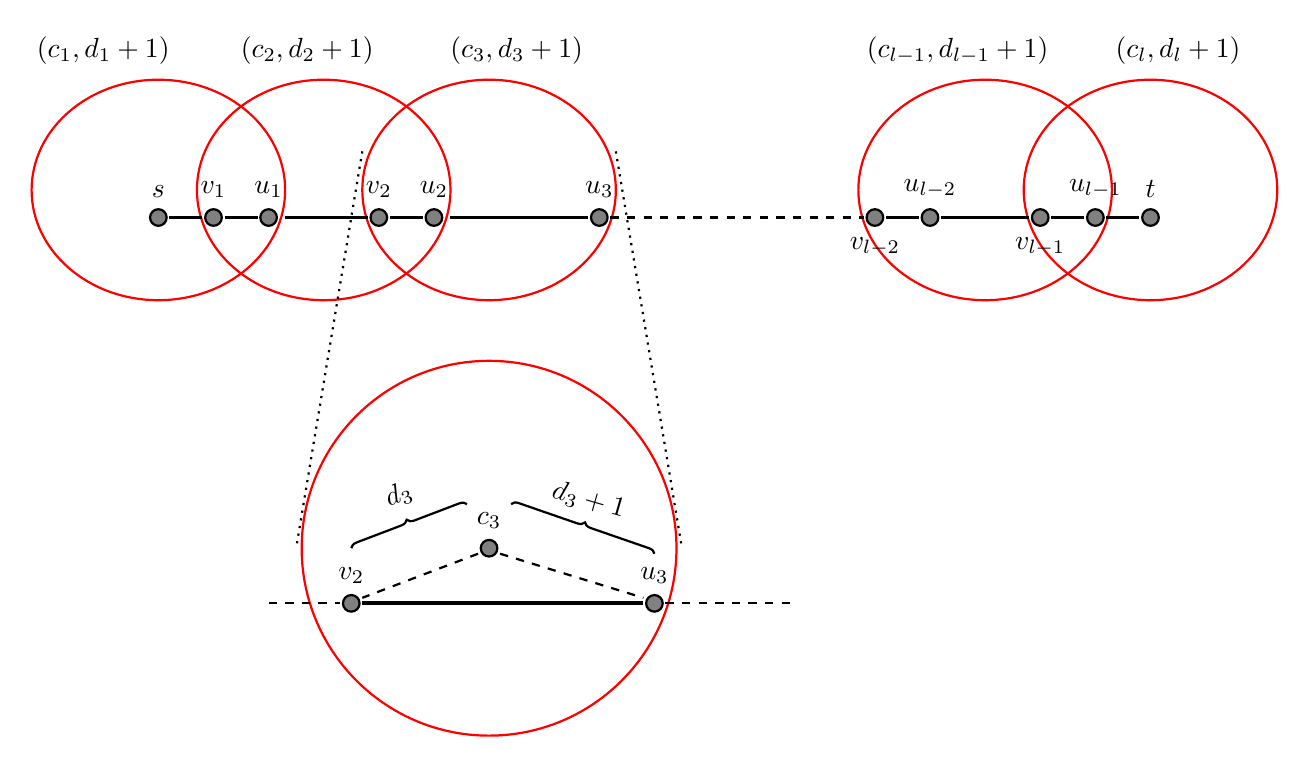
\begin{tikzpicture}[thick,scale=0.7]
	\draw [red] (15, 0.5) ellipse (2.3 and 2);
	\draw [red] (0, 0.5) ellipse (2.3 and 2);
	\draw [red] (3, 0.5) ellipse (2.3 and 2);
	\draw [red] (6, 0.5) ellipse (2.3 and 2);
	\draw [red] (18, 0.5) ellipse (2.3 and 2);
	
	\draw (0, 0) node[circle, draw, fill=black!50, inner sep=0pt, minimum width=6pt, label = $s$] {};
	\draw (18, 0) node[circle, draw, fill=black!50, inner sep=0pt, minimum width=6pt,label = $t$] {};
	
	\draw (2, 0) node[circle, draw, fill=black!50, inner sep=0pt, minimum width=6pt,label = $u_1$] {};
	\draw (1, 0) node[circle, draw, fill=black!50, inner sep=0pt, minimum width=6pt,label = $v_1$] {};
	\draw [line width = 0.5mm] (0.2, 0) -- (0.8, 0);
	\draw [line width = 0.5mm] (1.2, 0) -- (1.8, 0);
	
	\draw (-1, 2.4) node[red, label={$\ball(c_1, d_{1}+1)$}]{};
	
	\draw (5, 0) node[circle, draw, fill=black!50, inner sep=0pt, minimum width=6pt,label = $u_2$] {};
	\draw [line width = 0.5mm] (2.3, 0) -- (3.8, 0);
	\draw [line width = 0.5mm] (4.2, 0) -- (4.8, 0);
	
	\draw (2.7, 2.4) node[red, label={$\ball(c_2, d_{2}+1)$}]{};
	
	\draw (4, 0) node[circle, draw, fill=black!50, inner sep=0pt, minimum width=6pt,label = $v_2$] {};
	\draw (8, 0) node[circle, draw, fill=black!50, inner sep=0pt, minimum width=6pt,label = $u_3$] {};
	\draw [line width = 0.5mm] (5.3, 0) -- (7.8, 0);
	
	\draw (6.5, 2.4) node[red, label={$\ball(c_3, d_{3}+1)$}]{};
	
	\draw[dotted] (3.7, 1.2) -- (2.5, -6);
	\draw[dotted] (8.3, 1.2) -- (9.5, -6);
	\draw (3.5, -7) node[circle, draw, fill=black!50, inner sep=0pt, minimum width=6pt,label = $v_2$] {};
	\draw (9, -7) node[circle, draw, fill=black!50, inner sep=0pt, minimum width=6pt,label = $u_3$] {};
	\draw (6, -6) node[circle, draw, fill=black!50, inner sep=0pt, minimum width=6pt,label = $c_3$] {};
	\draw [red] (6, -6) ellipse (3.4 and 3.4);
	\draw [line width = 0.5mm] (3.7, -7) -- (8.8, -7);
	\draw [dashed] (2, -7) -- (3.3, -7);
	\draw [dashed] (9.2, -7) -- (11.5, -7);
		\draw [decorate,
	decoration = {brace}] (3.5,-6) -- (5.6,-5.2);
	\draw (4.5, -5.6) node[label={[rotate=20]$d_3$}]{};
	\draw [dashed] (5.8, -6.1) -- (3.7, -6.9);
	\draw [decorate,
	decoration = {brace}] (6.4,-5.2) -- (9,-6.1);
	\draw (7.7, -5.7) node[label={[rotate=-16]$d_3+1$}]{};
	\draw [dashed] (6.2, -6.1) -- (8.8, -6.9);
	
	\draw (16, 0) node[circle, draw, fill=black!50, inner sep=0pt, minimum width=6pt,label = -90: $v_{l-1}$] {};
	\draw (17, 0) node[circle, draw, fill=black!50, inner sep=0pt, minimum width=6pt,label = $u_{l-1}$] {};
	\draw [line width = 0.5mm] (17.8, 0) -- (17.2, 0);
	\draw [line width = 0.5mm] (16.8, 0) -- (16.2, 0);

	
	\draw (18.5, 2.4) node[red, label={$\ball(c_l, d_{l}+1)$}]{};
	
	\draw (13, 0) node[circle, draw, fill=black!50, inner sep=0pt, minimum width=6pt,label = -90 : $v_{l-2}$] {};
	\draw (14, 0) node[circle, draw, fill=black!50, inner sep=0pt, minimum width=6pt,label = $u_{l-2}$] {};
	\draw [line width = 0.5mm] (13.8, 0) -- (13.2, 0);
	\draw [line width = 0.5mm] (15.8, 0) -- (14.2, 0);
	
	\draw (14.5, 2.4) node[red, label={$\ball(c_{l-1}, d_{{l-1}}+1)$}]{};
	
	\draw [dashed] (8.2, 0) -- (12.8, 0);
\end{tikzpicture}